%!TEX root = ../main.tex
\chapter{Methods for Compton imaging\label{chap:mlem_theory}}
The 3D reconstruction of sources of ionizing radiation poses a challenging problem.
The difficulty of this task lies in the fact that the detected $\gamma$ particle could originate anywhere on the surface of the reconstructed Compton cone.
Several methods for Compton imagining have been investigated in the past.
This chapter provides a brief overview of such methods and describes the theoretical background of the \ac{MLEM} method.

\section{Compton imagining in nuclear medicine}
The problem of reconstructing 3D positions of sources of ionizing radiation has been studied in depth in the field of medical imaging, where it is used as a non-invasive method for diagnostics.
To give an example:
In cancer diagnostics, a small amount of radioactive substance (called a tracer) is injected into the patient's vein.
The tracer is absorbed by different parts of the body in varying amounts, which can show areas with abnormal metabolic activity, which is usually the case for cancer cells.
The detection of emitted particles and 3D reconstruction of their sources allow doctors to find the location of the tumour in the patient's body.

\section{Differences}
Compton imaging in medical applications typically requires a high resolution of the reconstructed image.
The distances between source and detector are small (tens of centimetres), number of measured events is high (tens of thousands and more).
The reconstruction process is typically performed offline (all measurements are collected first, and then the algorithms process the data) since there is no need for online estimation, and the processing of measured data might take non-negligible time.
The domain of multi-robot radiation mapping has multiple differences compared to the medical field.
The distance between the source and detector is much larger (from meters to hundreds of meters).
The \ac{UAV}s have limited payload (hence the detector carried on board must be light and compact).
It results in the fact that the number of measurements is much lower (hundreds-thousands detected Compton events).
Moreover, we would like to reconstruct the sources of ionizing radiation in real-time.
Despite all of these differences, the aim of this work is to get inspiration in the medical field and apply these algorithms to the given problem.

\section{Reconstruction methods}
The reconstruction methods can be divided into two categories: analytical (direct) and iterative algorithms \cite{lojacono2}.
\subsection{Analytical reconstruction methods}
In analytical methods, the aim is to find a solution directly from the conical projections of reconstructed Compton events.
Such a solution might be exact in the continuous model (e.g. computing the exact intersection point of all acquired Compton measurements), yet impractical in real-world applications, where the measurements might be noisy (thus, conical surface projections might not intersect the real position of the source) or where the computational power is limited.
To illustrate the difficulties of direct reconstruction methods, the algorithm proposed in \cite{baca2021gamma} estimates the initial hypothesis of the source position as a point that is closest to all measured cone surfaces (which might be considered an analytical method).
Finding a solution to the nonlinear least squares problem is computationally demanding and tractable only for a small number of cones.
Another example of a simple direct reconstruction method is called back-projection.
\subsubsection{Back-projection}
Back-projection is one of the simplest reconstruction methods. 
The Compton cones are projected to the (discretized) space of possible source locations, and each bin records the number of cones intersecting its position. 
The bins with more intersections are considered as possible source positions.
The back-projection for 2D image reconstruction is illustrated in  \autoref{fig:bppp}.
The advantage of back-projection method is its simplicity and the fact that it can be easily parametrized when processing a large number of measurements.
On the other hand, the back-projection requires a significant number of data in order to make the reconstruction accurate and does not take into account the properties of the detector.
  \begin{figure}[!h]
    \centering
      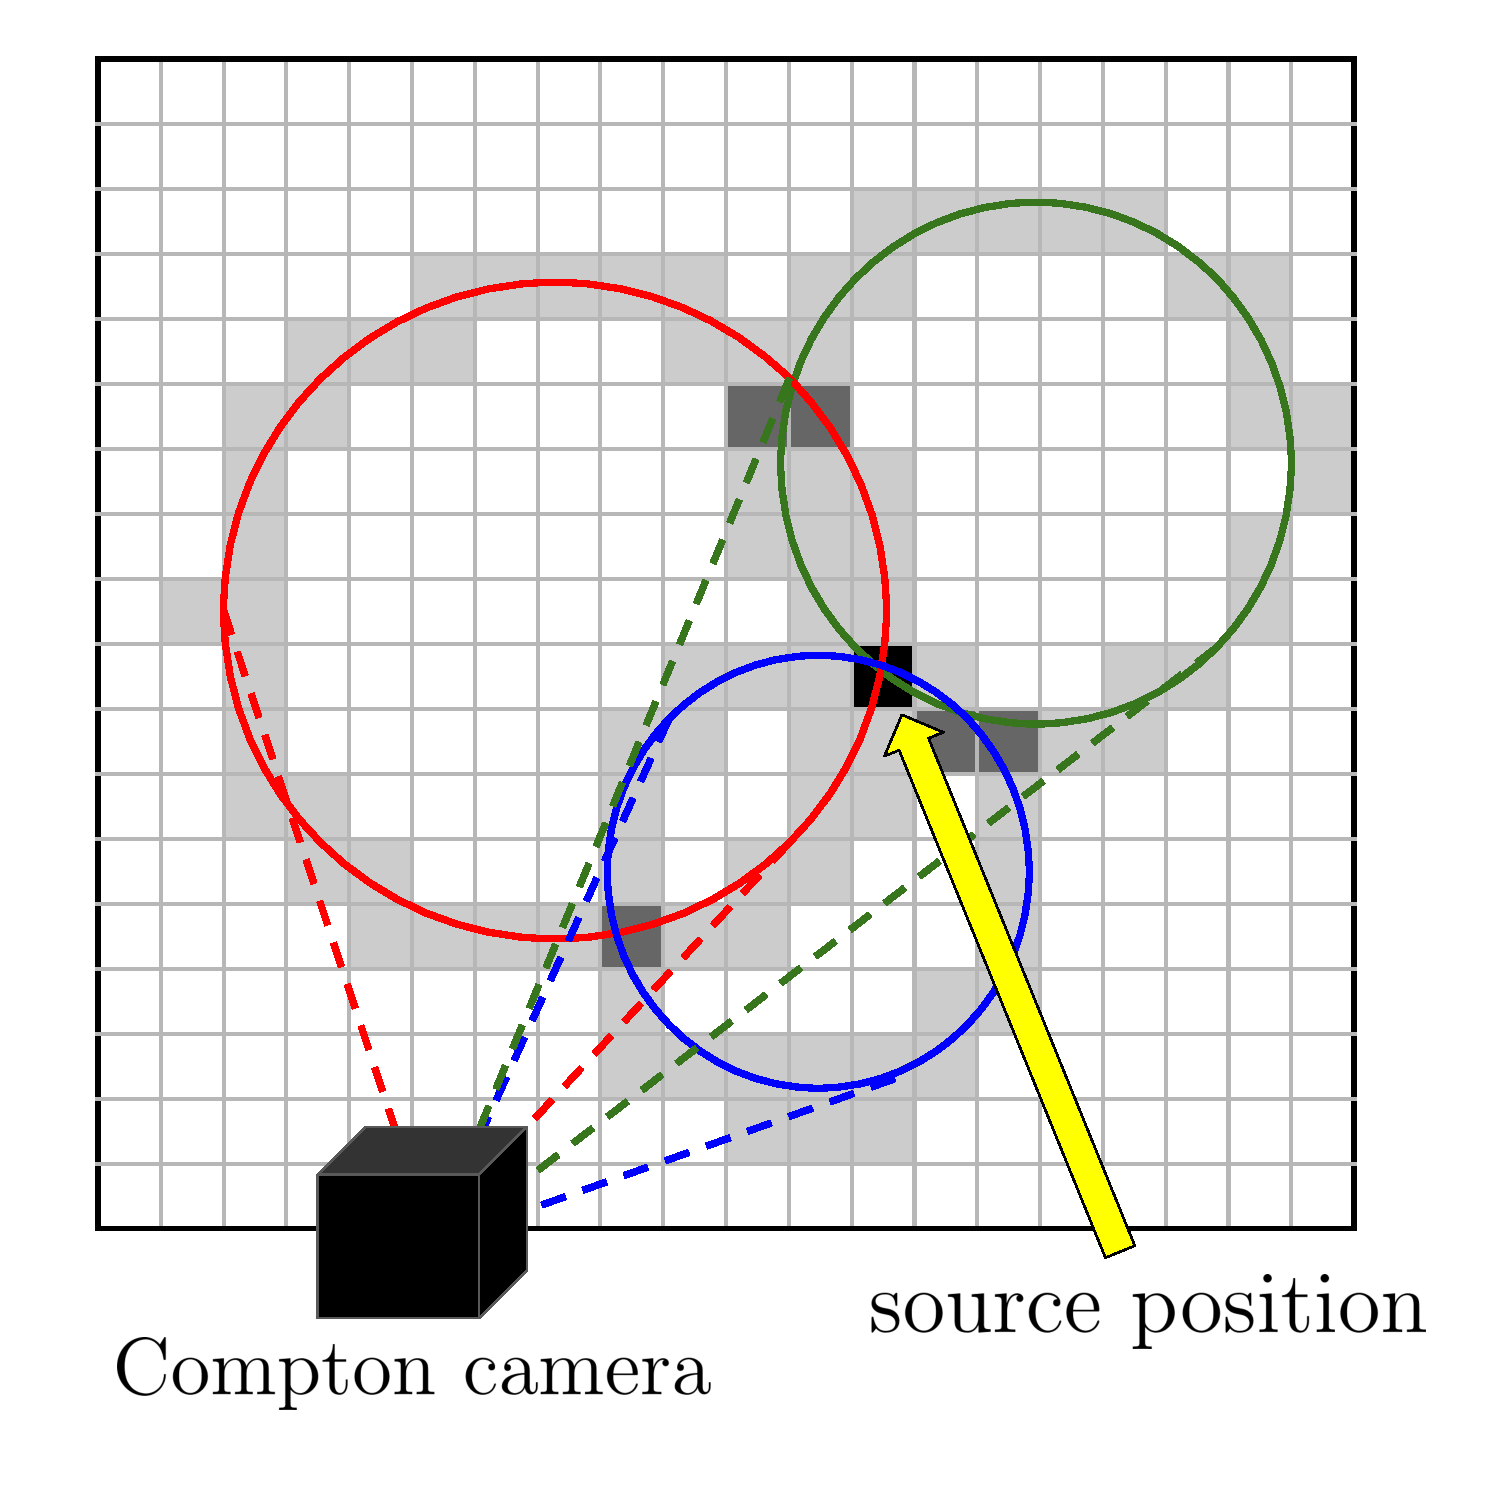
\includegraphics[width=0.5\textwidth]{./fig/photos/back_proppp.eps}
    \caption{Simple back-projection reconstruction method illustrated in 2D. Recorded Compton cones are back-projected to the space of possible source positions. The number of cones intersecting each bin is computed, as illustrated by the white-grey-black cell colours.}
    \label{fig:bppp}
  \end{figure}

\subsection{Iterative reconstruction methods}
The iterative reconstruction methods approximate the positions of sources by iteratively adapting the reconstruction to the measured projections.
Each iteration improves the current estimate based on the recorded measurements (the Compton cones), starting from some initial estimate or prior belief of sources distribution. 
The iterative approach does not provide an exact and unique solution. On the other hand, it is more flexible, can handle noise in the measurements (if it is properly modelled) and is widely used in practice.
The literature describes three main iterative reconstruction methods: \acf{MLEM}, \acf{MAP} and \acf{SOE}.
\ac{MLEM} \cite{MLEM_Shepp_1982}, \cite{MLEM_Lange_Carlson_1984}, \cite{MLEM_Wilderman_2000} is an iterative algorithm that is based on the maximum likelihood approach.
Another approach called \ac{MAP} \cite{MLEM_Lange_Carlson_1984} is based on the Bayesian approach.
It is an extension of \ac{MLEM} that allows to the incorporation of some prior knowledge about the source distribution or features of the data.
\ac{SOE} is a stochastic algorithm that randomly assigns the origins of the measured events to the conical surfaces.
During the course of reconstruction, the origins of events are stochastically moved, and the acceptance of the new event origin is determined by the change in event density.
After several iterations, the reconstructed distribution of origins converges to a quasistationary state \cite{SOE_Andreyev_2009}.

The iterative methods were originally developed for \ac{PET} and \ac{SPECT} imagining.
The \ac{PET}  method is based on positron emission. 
The emitted positron interacts with electrons in the patient's body, and both particles annihilate. 
The annihilation produces energy that comes in the form of two gamma photons that go in opposite directions.
Detection of these two gamma photons (measured by the detector at the same time) allows us to reconstruct a 3D image of the patient's body.
In \ac{SPECT}, only a single gamma ray is produced. 
Medical \ac{SPECT} imagining devices typically acquire measurements from different positions and use collimators to restrict the set of possible directions of incoming gamma radiation.
Measured events in \ac{PET} and \ac{SPECT} are stored in memory in discrete bins (each bin represents the count of reconstructed particles in a defined time interval or a subset of the image space).
The Compton camera events are represented in memory using the list-mode approach.
List-mode approach stores measured Compton cones in a list data structure, where each record contains information about the exact arrival time, position and energy of measured interactions.
Despite all these differences in the nature of the measurements, the iterative methods were also adapted for Compton imaging.

%Collimators restricts the set of possible directions from which the gamma ray may enter the detector (and be detected), therefore they can improve accuracy of the detection.
%Since only one gamma-ray is emmited (unlike in \ac{PET}), high number of measurements is needed for accute reconstruction.
%Medical \ac{SPECT} imagining cameras typically use collimators to get some information about direction of incoming gamma ray.
%Collimators restricts the set of possible directions from which the gamma ray may enter the detector (and be detected), therefore they can improve accuracy of the detection.

\section{Maximum likelihood expectation maximization}
The iterative \ac{MLEM} algorithm is widely used for image reconstruction from the Compton camera data. % \cite{maxim2016}.
The algorithm was originally proposed by \cite{MLEM_Shepp_1982} and later adapted to the Compton camera measurements and list-mode form by \cite{wilderman}.
As the name suggests, the algorithm is based on maximizing the likelihood of measured data.

\subsection{Maximum likelihood estimation}
\ac{MLE} is a classical approach in machine learning.
\ac{MLE} method is used to estimate the parameters of a probability distribution based on observed data. 
The goal of \ac{MLE} is to find the parameter values that make the observed data most probable under the assumed probability distribution.
This is done by calculating the likelihood function, which is the probability of the observed data given a set of parameter values.
The likelihood is defined as 
\begin{equation}
  \mathcal{L}(\boldsymbol{O}| \Phi) = P( \mathrm{observing\ measurements} \  \boldsymbol{O} \ \mathrm{given\ parameters\ } \Phi ).
  \label{eq:likelihood}
\end{equation}
We want to maximize this expression with respect to the hidden parameters.
In other words, we want to find such parameters that fit our observations in the best possible way.

\subsection{Original MLEM formulation}
Let us divide the area of possible sources of radiation into $J$ discrete bins (each indexed with $j$, where $j = 1 \dotsc J$).
%Each discrete bin is often represented by its centre position.
Suppose the binned data space of all measured events is $\mathbf{I}$, divided in $I$ discrete bins indexed with $i$, $i = 1 \dotsc I$.
The unobservable data space of all not measured events is denoted $\mathbf{\hat{I}}$.
Let us define the vector of measurements $\mathbf{Y}$ with elements $y_{i}$ ($i \in \{1, \dots I\}$) representing the number of particles detected in the corresponding bin $i$.
Let us define matrix $\mathbf{T}$ ($\mathbf{T} \in \mathbb{R}^{I \times J}$), where each position in the matrix is defined as
\begin{equation}
  t_{ij} =  P(\textrm{detected in } i | \textrm{emitted from } j).
\end{equation}
In other words, $t_{ij}$ represents the probability that we observe observation $i$ given that a radioactive particle that caused the observation $i$ has been emitted from position $j$.
Let us assume that the number of photons emitted from one position $j$ is a discrete random variable that follows a Poisson distribution with the expected value $\lambda_{j}$.
Our goal is to estimate vector $\bm{\lambda}$ with elements $\lambda_{j}$ ($j \in \{1 , \dots, J\}$), each corresponding to the expected intensity of emission from the position $j$.

%(the algorithm was originally developed for \ac{PET} imaging, where $y_{i}$ can be arbitrary number, $y_{i} = 1$ in list-mode representation).
Let us assume (for the purpose of the algorithm's derivation) that the matrix $\mathbf{T}$ is known.
Then a vector $\bm{\mu}$ can be defined, where each element of $\bm{\mu}$ 
\begin{equation}
  \mu_{i} = \sum_{j} t_{ij}\lambda_{j}
  \label{eq:mu}
\end{equation}
denotes the average number of events measured in bin $i$.
The probability of measuring $y_{i}$ particles in the measurement bin $i$ with respect to some given average emission intensity $\bm{\lambda}$ is then expressed as (Poisson distribution):
\begin{equation}
  p(y_{i} |\mu_{i} ) = e^{-\mu_{i}} \frac{\mu_{i}^{y_i}}{y_{i}!}.
\end{equation}
The likelihood of all the measurements (assuming the events to be independent) is
\begin{equation}  
  \mathcal{L}(\mathbf{Y} | \bm{\lambda}) = \prod_{i}p(y_{i} |\mu_{i} ) = \prod_{i} e^{-\mu_{i}} \frac{\mu_{i}^{y_i}}{y_{i}!}.
  \label{eq:prod}
\end{equation}
We want to maximize the likelihood by finding the best possible values of $\bm{\lambda}$. 
The maximum likelihood solution is:
\begin{equation}
  \bm{\lambda}_{best} = \underset{\bm{\lambda}}{\mathrm{argmax}}( \mathrm{log}\ \mathcal{L}(\mathbf{Y} | \bm{\lambda})).
\end{equation}
Instead of maximizing the product in equation \ref{eq:prod}, it is common to maximize its logarithm since the logarithm is a monotonically increasing function.
After taking the logarithm of \ref{eq:prod} and substitution $\mu_{i} = \sum_{j} t_{ij}\lambda_{j}$, we have the following:
\begin{equation}  
  \mathrm{log}\ \mathcal{L}(\mathbf{Y} | \mathbf{\lambda}) = \sum_{i}\left ( -\sum_{j} t_{ij}\lambda_{j} + y_{i} \mathrm{log}(\sum_{j} t_{ij}\lambda_{j})  - \mathrm{log}(y_{i}!) \right ).
  \label{eq:likelihood1}
\end{equation}
However, the nonlinear equation \ref{eq:likelihood1} can not be maximized directly.
The solution is to use an iterative \ac{EM} algorithm, as proposed in \cite{MLEM_Lange_Carlson_1984}.
\subsection{Expectation maximization algorithm}
The \ac{EM} algorithm was originally described in \cite{EM}. 
It is an iterative algorithm consisting of two steps performed in each iteration --- E-step and M-step.
The iterations of ac	
The vector of hidden parameters  $\mathbf{\hat{\lambda}}^{[l = 0]}$ we would like to find is initialized to some starting value using back-projection of the Compton cones or with uniform distribution.
The purpose of the E-step is to determine the expectation of the likelihood function given the measurements $\mathbf{Y}$ and the estimation of hidden parameters $\mathbf{\hat{\lambda}}^{[l-1]}$ obtained from the previous iteration. 
Then in the M-step, this expectation is maximized by setting its derivatives (with respect to $\mathbf{\hat{\lambda}}^{[l-1]}$) to $0$.
According to \cite{MLEM_Lange_Carlson_1984}, the final formula for iterative \ac{MLEM} algorithm with binned data is 
\begin{equation}
  \hat{\lambda}_{j}^{[l]} = \frac{\hat{\lambda}_{j}^{[l-1]}}{\sum_{i}t_{ij}} \sum_{i \in I} \frac{t_{ij} y_{i}}{\sum_{k} t_{ik} \hat{\lambda}_{k}^{[l-1]}}.
  \label{eq:mlem_class}
\end{equation}
The term $\sum_{i}t_{ij}$ is called sensitivity of detection $s_{j}$ and presents the probability that particle emitted at position $j$ is detected by the sensor:
\begin{equation}
  s_{j} = P(\textrm{detected by the sensor}\ | \textrm{emitted from } j) =  \sum_{i}t_{ij}.
\end{equation}
\subsection{List-mode Maximum Likelihood Expectation Maximization}
The list-mode extension of \ac{MLEM} for the Compton imaging was proposed in \cite{wilderman}.
Each measurement bin $i$ in list-mode \ac{MLEM} consists of only one detected Compton event.
Therefore the number of detected events $y_{i}$ in data bin $i$ is either $y_{i} = 1$ for the detected event or $y_{1} = 0$ when no event was recorded.
This simplifies the formula \ref{eq:mlem_class} to
\begin{equation}
  \hat{\lambda}_{j}^{[l]} = \frac{\hat{\lambda}_{j}^{[l-1]}}{s_{j}} \sum_{i \in \mathbf{I}}\frac{t_{ij} }{\sum_{k} t_{ik} \hat{\lambda}_{k}^{[l-1]}}.
  \label{eq:lmmlem}
\end{equation}
We denote as \ac{MLEM} the list-mode \ac{MLEM} algorithm for Compton imaging formulated in \ref{eq:lmmlem} in the rest of the thesis for simplicity.
Since only recorded measurements are considered in the list-mode approach, it no longer holds that sensitivity of measurements can be expressed as $s_{j} = \sum_{i}t_{ij}$ (summation over all measurement bins $i$).
The sensitivity of detection is then a sum over all events \{$\mathbf{I} \cup \mathbf{\hat{I}}\}$, not only those that were measured, therefore $s_{j} = \sum_{\mathbf{I} \cup \mathbf{\hat{I}}} t_{ij}$ for Compton imaging.
%The computational complexity of the \ac{MLEM} algorithm is $\mathcal{O}(I J)$
\subsection{MLEM algorithm in practical application}
The equation \ref{eq:lmmlem} presents the formulation of the iterative \ac{MLEM} algorithm maximizing the likelihood of measured data.
The system matrix $\mathbf{T}$ and vector of sensitivity values $\mathbf{s} \in \mathbb{R}^{J}$ with elements $s_{j}$ depend on the particular geometry of the used sensor and need to be derived individually in each application.
The description of system matrix $\mathbf{T}$ and sensitivity vector $\mathbf{s}$ adapted to the presented task is described in Chapter \ref{chap:methods_robotics}. 

Several other design choices are to be made in practical applications, such as setting the number of iterations of the \ac{MLEM} algorithm.
The number of iterations in \ac{MLEM} represents a balance between contrast recovery (quality of reconstruction) and image noise amplification, as stated in \cite{handheld_mlem_reconstruction}.
There is no general rule on how to set the optimal number of iterations --- it depends on the particular application, level of noise etc.
Therefore the number of iterations is set arbitrarily within this project based on the experiments with recorded real-world data.






%%%%%%%%%%%%%%%%%%%%%





%Another design-choice is the initialization of the vector $\mathbf{\hat{\lambda}}^[l = 0]$.



%Since the data for \ac{CC} are stored using list-mode approach, the $y_{i}$ (number of detected events in data bin $i$) in equation \ref{eq:mlem_class} is either $0$ or $1$.



%\section{Imagining in nuclear medicine}
%The problem of reconstructing 3D positions of sources of ionizing radiation has been studied in depth in the field of medical imagining.
%To give an example: one possible application of such methods is a cancer diagnostics.

%There are numerous methods used in medical imagining. 
%Two main approaches are following: \ac{PET} and \ac{SPECT}.
%\ac{PET} imagining typically use a gamma emitting radioisotope as a tracer.  
%The method is based on positron emission. 
%The emitted positron interacts with electron in the patients body and both particles vanish in a burst of energy. 
%This energy comes in a form of two gamma rays, that goes into a opposite directions.
%Detection of these two gamma rays (measured by the camera at the same time) allows us to reconstruct 3D image of the patient's body.
%In \ac{SPECT}, single gamma ray is produced. 
%The reconstructed image is computed from gamma rays detected by the camera.
%Since only one gamma-ray is emmited (unlike in \ac{PET}), high number of measurements is needed for accute reconstruction.
%Medical \ac{SPECT} imagining cameras typically use collimators to get some information about direction of incoming gamma ray.
%Collimators restricts the set of possible directions from which the gamma ray may enter the detector (and be detected), therefore they can improve accuracy of the detection.

%Another type of sensor (that can be used in \ac{SPECT} imagining) is a Compton camera.
%The biggest benefit of compton camera is that it provides information about the direction of detected incoming gamma ray without the use of collimator.
%The nuclear medicine reconstruction method for compton camera measurements that served as inspiration for for this thesis is called \ac{LM-MLEM}.
